\begin{figure}[H]
    \centering
    \resizebox{0.5\linewidth}{!}{
    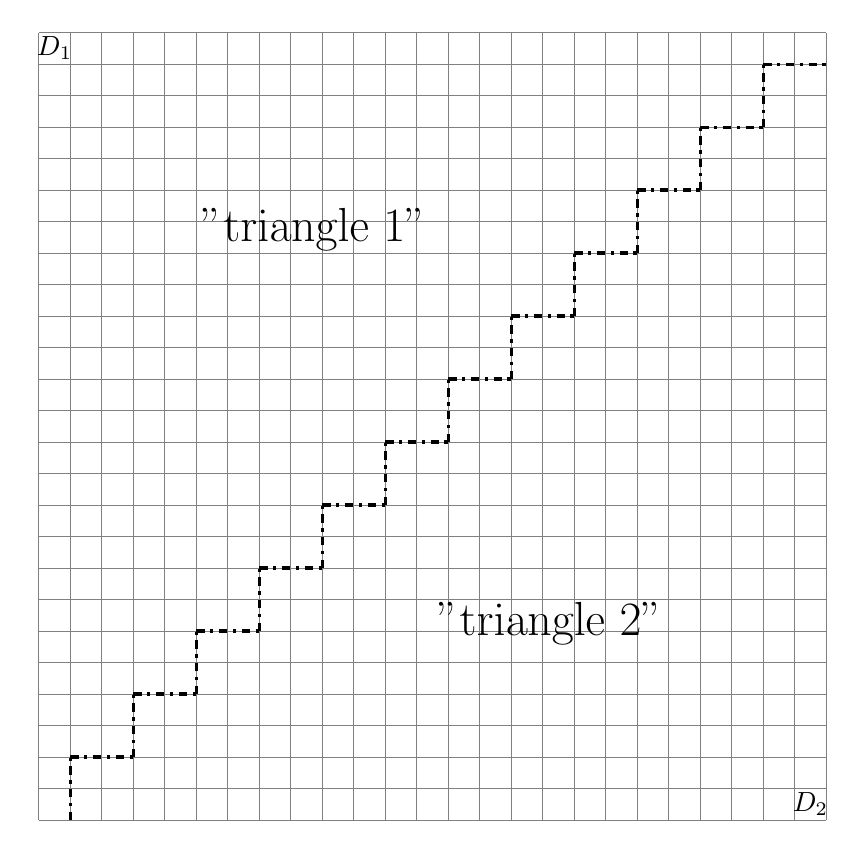
\begin{tikzpicture}
        \draw[step=0.4cm,color=gray] (0,0) grid (10,10);
        \node at (0.2,9.8) {$D_1$};
        \node at (9.8,0.2) {$D_2$};
        \node at (3.5,7.5) {\LARGE "triangle 1"};
        \node at (6.5,2.5) {\LARGE "triangle 2"};
        \draw[very thick, dash dot] (9.2,9.6) -- (10.0,9.6);
        \draw[very thick, dash dot] (9.2,8.8) -- (9.2,9.6);
        \draw[very thick, dash dot] (8.4,8.8) -- (9.2,8.8);
        \draw[very thick, dash dot] (8.4,8.0) -- (8.4,8.8);
        \draw[very thick, dash dot] (7.6,8.0) -- (8.4,8.0);
        \draw[very thick, dash dot] (7.6,7.2) -- (7.6,8.0);
        \draw[very thick, dash dot] (6.8,7.2) -- (7.6,7.2);
        \draw[very thick, dash dot] (6.8,6.4) -- (6.8,7.2);
        \draw[very thick, dash dot] (6.0,6.4) -- (6.8,6.4);
        \draw[very thick, dash dot] (6.0,5.6) -- (6.0,6.4);
        \draw[very thick, dash dot] (5.2,5.6) -- (6.0,5.6);
        \draw[very thick, dash dot] (5.2,4.8) -- (5.2,5.6);
        \draw[very thick, dash dot] (4.4,4.8) -- (5.2,4.8);
        \draw[very thick, dash dot] (4.4,4.0) -- (4.4,4.8);
        \draw[very thick, dash dot] (3.6,4.0) -- (4.4,4.0);
        \draw[very thick, dash dot] (3.6,3.2) -- (3.6,4.0);
        \draw[very thick, dash dot] (2.8,3.2) -- (3.6,3.2);
        \draw[very thick, dash dot] (2.8,2.4) -- (2.8,3.2);
        \draw[very thick, dash dot] (2.0,2.4) -- (2.8,2.4);
        \draw[very thick, dash dot] (2.0,1.6) -- (2.0,2.4);
        \draw[very thick, dash dot] (1.2,1.6) -- (2.0,1.6);
        \draw[very thick, dash dot] (1.2,0.8) -- (1.2,1.6);
        \draw[very thick, dash dot] (0.4,0.8) -- (1.2,0.8);
        \draw[very thick, dash dot] (0.4,0.0) -- (0.4,0.8);
    \end{tikzpicture}}
    \caption{'Grid' environment. The dotted lines have no effect on the environment, they simply separate the grid positions part of 'triangle 1' and 'triangle 2'.}
    \label{fig:grid}
\end{figure}